\documentclass{../../template/labo}

\usepackage[utf8x]{inputenc}
\usepackage[T1]{fontenc}
\usepackage{charter}
\usepackage{ucs}
\usepackage{amsthm} %numéroter les questions
\usepackage[frenchb]{babel}
\usepackage{datetime}
\usepackage{xspace} % typographie IN
\usepackage{hyperref}% hyperliens
\usepackage[all]{hypcap} %lien pointe en haut des figures
\usepackage[french]{varioref} %voir x p y
\usepackage{fancyhdr}% en têtes
\usepackage[]{graphicx} %include pictures
% \usepackage{pgfplots}
\usepackage[americanresistors,siunitx]{circuitikz}
\usepackage[]{gnuplottex}
\usepackage{ifthen}
\usepackage{mathastext} % math as standfard text : units are respecting typography conventions.
\usepackage[]{subfig}
\usepackage[]{attachfile}
\usepackage{tikz}
\usetikzlibrary{babel,positioning,calc}
\usepackage{siunitx}
\usepackage{amssymb}
\usepackage{xcolor}
\usepackage{float}
\usepackage[normalem]{ulem}
\usepackage{todonotes}

%%%%%%%%%%%%
% Tables
%%%%%%%%%%%%
\usepackage{booktabs}
\renewcommand{\arraystretch}{1.1} % Opens up the table a tad
\usepackage{multicol}
\usepackage{multirow}

\newboolean{koriG}
\ifx\koriG\undefined
\correction{false}
\else
\correction{true}
\fi

\newcommand{\itgv}[1]{\ifthenelse{\boolean{corrige}}{{\color{blue}#1}}{}} %si corrigé vrai...
\newcommand{\ifgv}[1]{\ifthenelse{\boolean{corrige}}{}{#1}} %si corrigé vrai...

% \correction{false}
%\correction{true}

\definecolor{darkblue}{rgb}{0,0,0.5}

%% fancy header & foot
\pagestyle{fancy}
\lhead{[AE3T] Laboratoire d'électronique appliquée\\ Labo 1~: Redresseur/doubleur}
\rhead{v1.0.0 \\ page \thepage}
\chead{\ifthenelse{\boolean{corrige}}{Corrigé}{}}
\cfoot{}
%%

\author{GEI}


\setlength{\parindent}{0pt}


%from SO: kinky cross for wires
\tikzset{
  declare function={% in case of CVS which switches the arguments of atan2
    atan3(\a,\b)=ifthenelse(atan2(0,1)==90, atan2(\a,\b), atan2(\b,\a));},
  kinky cross radius/.initial=+.125cm,
  @kinky cross/.initial=+, kinky crosses/.is choice,
  kinky crosses/left/.style={@kinky cross=-},kinky crosses/right/.style={@kinky cross=+},
  kinky cross/.style args={(#1)--(#2)}{
    to path={
      let \p{@kc@}=($(\tikztotarget)-(\tikztostart)$),
          \n{@kc@}={atan3(\p{@kc@})+180} in
      -- ($(intersection of \tikztostart--{\tikztotarget} and #1--#2)!%
             \pgfkeysvalueof{/tikz/kinky cross radius}!(\tikztostart)$)
      arc [ radius     =\pgfkeysvalueof{/tikz/kinky cross radius},
            start angle=\n{@kc@},
            delta angle=\pgfkeysvalueof{/tikz/@kinky cross}180 ]
      -- (\tikztotarget)}}}


\begin{document}
\tptitle{}{Labo 1~: Redresseur et doubleur de tension}

\section{Introduction}
L'objectif principal de ces manipulation est d'illustrer différentes utilisations des diodes.
Dans un premier temps, vous vous replongerez dans une application qui vous est familière : le circuit redresseur de tension. Il s'agira cependant d'une version améliorée réduisant certaines imperfections rencontrées dans sa version de base.
Vous manipulerez ensuite un circuit 555 afin de générer un signal carré périodique et doublerez la tension obtenue à l'aide d'un montage de Greinacher.

% \subsection{But de la manipulation et objectifs d'apprentissage}
% Cette manipulation a pour but d'illustrer :
% \begin{itemize}
% \item 
% \end{itemize}~\\

À la fin de ce laboratoire, vous devez être capable de :
\begin{itemize}
\item Déterminer les signaux permettant de mettre en évidence le comportement d'un circuit.
\item Déterminer la tension d'alimentation d'un circuit nécessaire à son bon fonctionnement.
\item Dimensionner un redresseur de précision simple ou double alternance avec ou sans gain.
\item Lire et comprendre une datasheet afin de déterminer le comportement et le dimensionnement d'un montage utilisant un circuit intégré (exemple : 555).
\item Comprendre et expliquer le fonctionnement d'un circuit doubleur de tension.
\end{itemize}

\subsection{Matériel}

\begin{center}
	\begin{tabular}{p{0.2\textwidth}rlp{0.1\textwidth}}
		Composant & \multicolumn{2}{c}{Valeur} & Quantité \\\toprule
		\multirow{1}{*}{AOP} & LM358 & & x1 \\\midrule
		\multirow{1}{*}{Diode} & 1N4148 & & x2 \\\midrule
		\multirow{1}{*}{Résistance} 	& 1 & k$\Omega$ & x3 \\\midrule
		\multirow{1}{*}{Résistance} 	& 10 & k$\Omega$ & x1 \\\midrule
		\multirow{1}{*}{Résistance} 	& 4.7 & k$\Omega$ & x1 \\\midrule
		\multirow{1}{*}{Résistance} 	& 39 & k$\Omega$ & x1 \\\midrule
		\multirow{1}{*}{Résistance} 	& 1 & M$\Omega$ & x1 \\\midrule
		\multirow{1}{*}{Condensateur} 	& 10 & nF & x2 \\\midrule
		\multirow{1}{*}{Condensateur} 	& 33 & \textmu F & x2 \\\midrule
		\multirow{1}{*}{Condensateur} 	& 1 & mF & x2 \\\bottomrule
	\end{tabular}
\end{center}

\section{Redresseur de précision (45 minutes)}
La diode peut être utilisée pour réaliser un redresseur de tension simple ou double alternance.
Dans le premier cas, seules les alternances \textit{positives} du signal sont conservées, tandis que dans le deuxième cas, les alternances négatives sont inversées afin d'être positives à leur tour.
Ce type de circuit est généralement utilisé lorsqu'on souhaite convertir une tension alternative en une tension continue, par exemple dans une alimentation.

Il est possible d'améliorer le montage en lui adjoignant un amplificateur opérationnel (AOP).
\begin{center}
	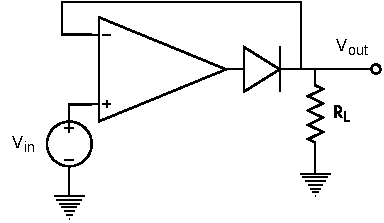
\includegraphics[width=.5\textwidth]{precision-rectifier.pdf}
\end{center}


\Question{
Réalisez le montage redresseur simple alternance de précision.
Utilisez un AOP LM358, une diode 1N4148 et une résistance $R_L = 1 k\Omega$.
Quel signal d'entrée allez-vous utiliser ?
Comment allez-vous alimenter l'AOP ?

}
{
Utiliser une simple sinusoïde de 1 V d'amplitude comme signal d'entrée, peu importe la fréquence.
L'AOP peut être alimenté en $\pm5 V$, mais ce n'est pas très important non plus.

Note : le sens de la diode en rétroaction détermine quelle alternance est redressée. Avec la cathode sur la sortie, on garde les alternances négatives non-redressées, avec l'anode sur la sortie, on garde les alternances positives.
}

\Question{
Quelle différence observez-vous par rapport à un redresseur simple alternance «~classique~» (sans AOP) ?
}
{
La tension de sortie redressée n'est pas diminuée de la tension de seuil de la diode.
}


On peut aller plus loin en ajoutant un gain au montage existant~:
\begin{center}
	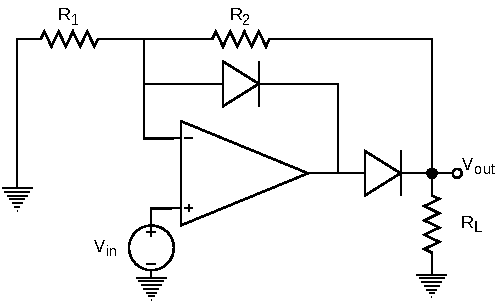
\includegraphics[width=.7\textwidth]{precision-rectifier-gain.pdf}
\end{center}

\Question{
Quelle est l'expression du gain de ce montage ?
}
{
Vout = -R2/R1
Les alternances négatives sont redressées et amplifiées.
}

\Question{
Réalisez le montage en utilisant une résistance $R_2$ de $10 k\Omega$ et une résistance $R_1$ de $1 k\Omega$ et $R_L$ de $1 k\Omega$. Quel gain observez-vous ?
}
{
-10.
Attention à bien choisir une tension d'entrée qui ne sature pas en fonction des alimentations choisies.
}

En profitant du fait qu'on a deux AOP dans un seul package de LM358, on peut facilement construire un redresseur double alternance de précision :
\begin{center}
	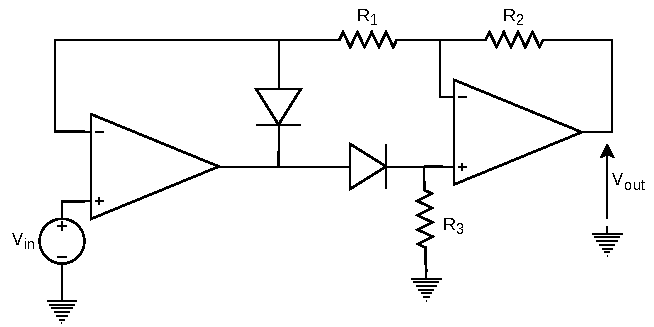
\includegraphics[width=.7\textwidth]{precision-rectifier-double.pdf}
\end{center}

\Question{
Réalisez le montage en utilisant des résistances de $1 k\Omega$ et observez la forme de la tension de sortie.
}
{

}



\clearpage







%%%%%%%%%%%%%%%%%%%%%%%%
% 555
%%%%%%%%%%%%%%%%%%%%%%%%
\section{Circuit à base de 555 (2 h 15)}
Cette partie met en œuvre le circuit intégré SE555\footnote{datasheet : \url{https://www.ti.com/lit/ds/symlink/se555.pdf}}. Ce circuit permet de facilement produire un signal carré alternatif à partir d'une alimentation continue. De nombreuses applications\footnote{\url{http://www.555-timer-circuits.com/}} ainsi qu'un concours annuel de design \footnote{\url{https://hackaday.io/contest/182830-555-timer-contest}} lui sont dédiés.


\subsection{Situation/problème}

L'application de cette manipulation consiste à doubler la tension continue utilisée pour alimenter notre circuit. Le circuit complet est représenté sur la Figure \ref{Doubleur} et est composé de deux blocs essentiels~:
\begin{enumerate}
	\item Un circuit 555 en mode \textit{astable} permettant de générer un signal carré périodique entre 0 et 5 V.
	\item Un montage de Greinacher légèrement modifié redressant et doublant la tension à son entrée.
\end{enumerate}

\begin{figure}[ht]
\centering
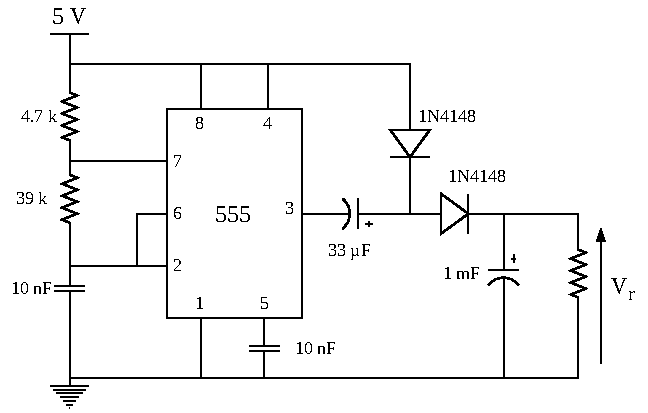
\includegraphics[width=0.8\textwidth]{555-doubler.pdf}
\caption{Circuit du doubleur de tension avec un timer 555}
\label{Doubleur}
\end{figure}


\subsection*{Préparation théorique}

\Question{
Sur base de la datasheet du timer et des composants présents dans le schéma :
\begin{itemize}
    \item Calculer et représenter graphiquement la période du signal carré qui sera produit par le 555 pour une tension Vin de 5V (Pin 4 \& 8)
    \item Définir le comportement global du circuit
    \item Exprimer $V_r$ (la tension aux bornes de la résistance) en fonction de la tension d'alimentation de 5 V \footnote{Allez-vous obtenir 10 V en sortie ?}. 
\end{itemize}
}{
Réponse attendue : relation globale du doubleur de tension et de ses pertes, notamment dues à la tension de seuil des diodes.
En utilisant des diodes Shottky (par exemple 1N5817), on atteint quasiment 10 V en sortie.

$V_r = 2 \times V_{in} - 2 \times V_{th} - V_{perte SE555}$
}


\subsection*{Manipulations}
Dans un premier temps, vous allez réaliser sur breadboard le schéma de la Figure \ref{NE555} avec une tension d'alimentation de 5V. 

\begin{figure}[ht]
\centering
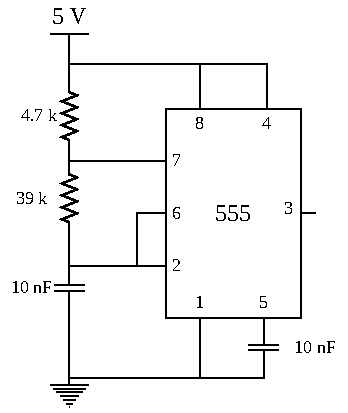
\includegraphics[width=0.35\textwidth]{555.pdf}
\caption{Circuit du 555 en mode astable.}
\label{NE555}
\end{figure}

\Question{
\begin{itemize}
	\item Quelle pin est la sortie du 555 ?
	\item Quel signal obtenez-vous à cette sortie ?
	\item Comparez votre mesure avec votre préparation théorique. Est-ce cohérent ? Expliquez !
\end{itemize}
}
{
	Sortie sur la pin 3.
}


Réalisez ensuite le schéma de la Figure \ref{Doubleur2} sur la même breadboard \textbf{sans la connecter} à la sortie du 555. Le signal $V_{in}$ est issu du générateur de signal : un signal carré de la même valeur de tension obtenue à la question précédente.
Dans un premier temps, utilisez une résistance de $1 M\Omega$ en sortie du montage.




\begin{figure}[ht]
\centering
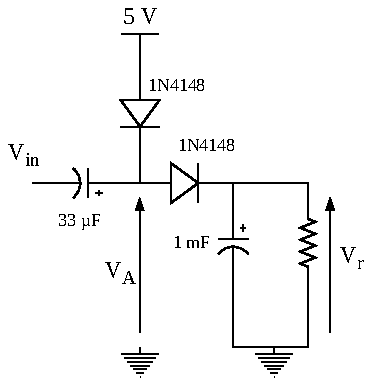
\includegraphics[width=0.4\textwidth]{doubler.pdf}
\caption{Circuit du doubleur de tension seul.}
\label{Doubleur2}
\end{figure}

\Question{
Quelle tension obtenez-vous pour $V_A$ ? Cela correspond-il à votre estimation théorique ?
}
{

}

\Question{
Quelle tension $V_r$ obtenez-vous en sortie ?  Cela correspond-il à votre estimation théorique ?
}
{

}


Finalement, connectez la sortie du 555 au doubleur de tension.


\Question{
Obtenez-vous la même Tension $V_r$ que celle obtenue à l'étape précédente ? 
}
{

}


\Question{
Quelle charge minimale pouvez-vous connecter à votre sortie ? Faites une estimation expérimentalement.
}
{

}


\Question{
Discutez du comportement général du circuit
}
{

}

% \Question{

% }
% {

% }

% \begin{astuce}
% \end{astuce}

\end{document}
